\section{Definição do Problema} \label{sec:problem}

Para delimitar o escopo do problema, primeiro: elementos ativos não serão
considerados (ex.: terminal de linha óptico); segundo: uma fibra será
considerada ocupada (isto é, alocada) caso haja um comprimento de onda
associado a ela, ao longo desse artigo, vamos considerar apenas um comprimento
de onda por alocação (multiplexação por divisão de onda não será considerado);
terceiro: desconsidera-se atenuação; quarto: desconsidera-se o uso de
splitters, onde um mesmo comprimento de onda em uma fibra é "espalhado" para
$n$ fibras em um nó.

Fazendo um palalelo com \cite{artigorwa} e \cite{zang2000review}, podemos notar
a menção de "conversores ópticos", em uma aplicação mais genérica. O presente
artigo é um "subconjunto" do tema de alocação e roteamento de onda tratado nas
referências citadas.

Em uma rede recém implementada, com zero alocações de sinal, boa parte dos tubos 
nas caixas ainda não foram abertos. Quando há mudança de capacidade de cabos nas
caixas, as fibras geralmente são "espelhadas". Uma alocação de fibras ótima
seria do índice menor das fibras até o maior índice, ou vice-versa.

Algumas situações que podem surgir ao longo do tempo são, por exemplo, em um
rompimento de rede, a troca temporária de um trecho por um cabo de menor 
capacidade. A Figura \ref{fig:fluxo_reduzido} mostra como as alocações de sinal
perdem o "espelhamento", porém note que os sinais retornam para o mesmo índice
no cabo seguinte, isso facilita muito ao trocar o cabo temporário por outro de
maior capacidade.

\begin{figure}
  \centering
  \caption{fluxo reduzido}
  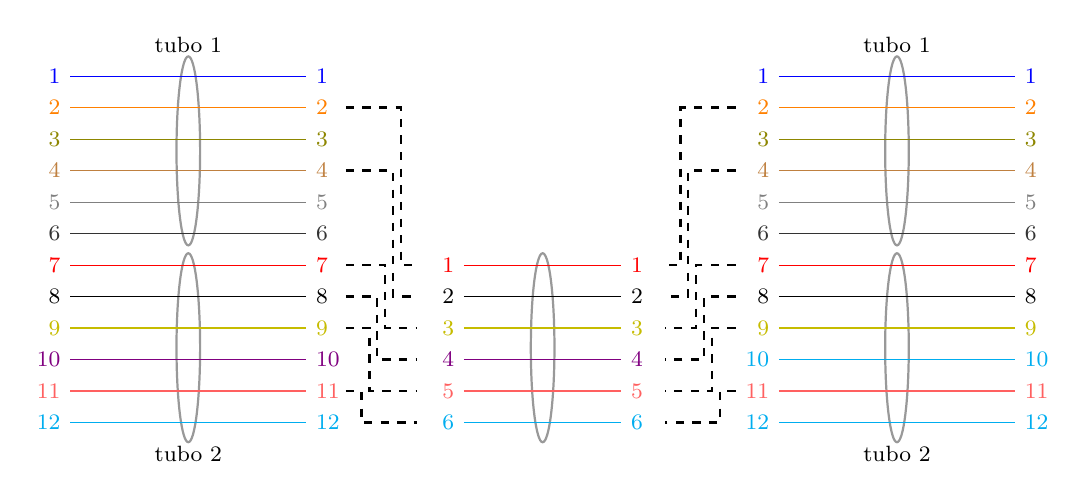
\begin{tikzpicture}[font=\footnotesize]
    % cabo 01
    \node at (1.5,-4mm) {tubo 2};
    \draw[gray!80, thick] (1.5,9.5mm) ellipse [x radius=1.5mm, y radius=12mm];
    \draw[cyan] (0,0mm) node[align=left,left] {12} -- (3,0mm) node[align=right,right] {12};
    \draw[pink!50!red] (0,4mm) node[align=left,left] {11} -- (3,4mm) node[align=right,right] {11};
    \draw[violet] (0,8mm) node[align=left,left] {10} -- (3,8mm) node[align=right,right] {10};
    \draw[yellow!50!olive] (0,12mm) node[align=left,left] {9} -- (3,12mm) node[align=right,right] {9};
    \draw[black] (0,16mm) node[align=left,left] {8} -- (3,16mm) node[align=right,right] {8};
    \draw[red] (0,20mm) node[align=left,left] {7} -- (3,20mm) node[align=right,right] {7};

    \node at (1.5,48mm) {tubo 1};
    \draw[gray!80, thick] (1.5,34.5mm) ellipse [x radius=1.5mm, y radius=12mm];
    \draw[black!80] (0,24mm) node[align=left,left] {6} -- (3,24mm) node[align=right,right] {6};
    \draw[gray] (0,28mm) node[align=left,left] {5} -- (3,28mm) node[align=right,right] {5};
    \draw[brown] (0,32mm) node[align=left,left] {4} -- (3,32mm) node[align=right,right] {4};
    \draw[olive] (0,36mm) node[align=left,left] {3} -- (3,36mm) node[align=right,right] {3};
    \draw[orange] (0,40mm) node[align=left,left] {2} -- (3,40mm) node[align=right,right] {2};
    \draw[blue] (0,44mm) node[align=left,left] {1} -- (3,44mm) node[align=right,right] {1};

    % fusões cabo 01 - cabo 02
    \draw[dashed,thick] (3.5,4mm) -- (3.7,4mm) -- (3.7,0mm) -- (4.4,0mm);
    \draw[dashed,thick] (3.5,12mm) -- (3.8,12mm) -- (3.8,4mm) -- (4.4,4mm);
    \draw[dashed,thick] (3.5,16mm) -- (3.9,16mm) -- (3.9,8mm) -- (4.4,8mm);
    \draw[dashed,thick] (3.5,20mm) -- (4.0,20mm) -- (4.0,12mm) -- (4.4,12mm);
    \draw[dashed,thick] (3.5,32mm) -- (4.1,32mm) -- (4.1,16mm) -- (4.4,16mm);
    \draw[dashed,thick] (3.5,40mm) -- (4.2,40mm) -- (4.2,20mm) -- (4.4,20mm);

    % cabo 02
    \draw[gray!80, thick] (6,9.5mm) ellipse [x radius=1.5mm, y radius=12mm];
    \draw[cyan] (5,0mm) node[align=left,left] {6} -- (7,0mm) node[align=right,right] {6};
    \draw[pink!50!red] (5,4mm) node[align=left,left] {5} -- (7,4mm) node[align=right,right] {5};
    \draw[violet] (5,8mm) node[align=left,left] {4} -- (7,8mm) node[align=right,right] {4};
    \draw[yellow!50!olive] (5,12mm) node[align=left,left] {3} -- (7,12mm) node[align=right,right] {3};
    \draw[black] (5,16mm) node[align=left,left] {2} -- (7,16mm) node[align=right,right] {2};
    \draw[red] (5,20mm) node[align=left,left] {1} -- (7,20mm) node[align=right,right] {1};

    % fusões cabo 01 - cabo 02
    \begin{scope}[xscale=-1,xshift=-340]
      \draw[dashed,thick] (3.5,4mm) -- (3.7,4mm) -- (3.7,0mm) -- (4.4,0mm);
      \draw[dashed,thick] (3.5,12mm) -- (3.8,12mm) -- (3.8,4mm) -- (4.4,4mm);
      \draw[dashed,thick] (3.5,16mm) -- (3.9,16mm) -- (3.9,8mm) -- (4.4,8mm);
      \draw[dashed,thick] (3.5,20mm) -- (4.0,20mm) -- (4.0,12mm) -- (4.4,12mm);
      \draw[dashed,thick] (3.5,32mm) -- (4.1,32mm) -- (4.1,16mm) -- (4.4,16mm);
      \draw[dashed,thick] (3.5,40mm) -- (4.2,40mm) -- (4.2,20mm) -- (4.4,20mm);
    \end{scope}

    % cabo 03
    \node at (10.5,-4mm) {tubo 2};
    \draw[gray!80, thick] (10.5,9.5mm) ellipse [x radius=1.5mm, y radius=12mm];
    \draw[cyan] (9,0mm) node[align=left,left] {12} -- (12,0mm) node[align=right,right] {12};
    \draw[pink!50!red] (9,4mm) node[align=left,left] {11} -- (12,4mm) node[align=right,right] {11};
    \draw[cyan] (9,8mm) node[align=left,left] {10} -- (12,8mm) node[align=right,right] {10};
    \draw[yellow!50!olive] (9,12mm) node[align=left,left] {9} -- (12,12mm) node[align=right,right] {9};
    \draw[black] (9,16mm) node[align=left,left] {8} -- (12,16mm) node[align=right,right] {8};
    \draw[red] (9,20mm) node[align=left,left] {7} -- (12,20mm) node[align=right,right] {7};

    \node at (10.5,48mm) {tubo 1};
    \draw[gray!80, thick] (10.5,34.5mm) ellipse [x radius=1.5mm, y radius=12mm];
    \draw[black!80] (9,24mm) node[align=left,left] {6} -- (12,24mm) node[align=right,right] {6};
    \draw[gray] (9,28mm) node[align=left,left] {5} -- (12,28mm) node[align=right,right] {5};
    \draw[brown] (9,32mm) node[align=left,left] {4} -- (12,32mm) node[align=right,right] {4};
    \draw[olive] (9,36mm) node[align=left,left] {3} -- (12,36mm) node[align=right,right] {3};
    \draw[orange] (9,40mm) node[align=left,left] {2} -- (12,40mm) node[align=right,right] {2};
    \draw[blue] (9,44mm) node[align=left,left] {1} -- (12,44mm) node[align=right,right] {1};
  \end{tikzpicture}
	\label{fig:fluxo_reduzido}
\end{figure}

Outro ponto de relevância na elaboração de qualquer algoritmo para tratar do
problema do presente artigo, é o fato de que alocação de fibras é um problema
NP-completo. É trivial comprovar isso, pois da mesma forma que o problema do
caixeiro-viajante \cite{lawler1985travelling} é fatorial com cada cidade
adicionada, para cada par de fibra adicionado, as combinações crescem em
$O(n!)$. A Figura \ref{fig:combinacoes_possiveis} ilustra todas as combinações
possíveis para três pares de fibra.

- fazer comparativo com o problema de otimização de fluxo máximo;

\begin{figure}
  \centering
  \caption{Combinações possíveis para 3 pares de fibra}
  \begin{tikzpicture}[font=\footnotesize]
    \graph [branch down=5mm] {
      subgraph I_nm [n=3, m=3];
      V 1 -- [blue] W 1;
      V 2 -- [orange] W 2;
      V 3 -- [olive] W 3;
    };
    \begin{scope}[xshift=2cm]
      \graph [branch down=5mm] {
        subgraph I_nm [n=3, m=3];
        V 1 -- [blue] W 2;
        V 2 -- [orange] W 1;
        V 3 -- [olive] W 3;
      };
    \end{scope}
    \begin{scope}[xshift=4cm]
      \graph [branch down=5mm] {
        subgraph I_nm [n=3, m=3];
        V 1 -- [blue] W 1;
        V 2 -- [orange] W 3;
        V 3 -- [olive] W 2;
      };
    \end{scope}
    \begin{scope}[xshift=6cm]
      \graph [branch down=5mm] {
        subgraph I_nm [n=3, m=3];
        V 1 -- [blue] W 3;
        V 2 -- [orange] W 1;
        V 3 -- [olive] W 2;
      };
    \end{scope}
    \begin{scope}[xshift=8cm]
      \graph [branch down=5mm] {
        subgraph I_nm [n=3, m=3];
        V 1 -- [blue] W 2;
        V 2 -- [orange] W 3;
        V 3 -- [olive] W 1;
      };
    \end{scope}
    \begin{scope}[xshift=10cm]
      \graph [branch down=5mm] {
        subgraph I_nm [n=3, m=3];
        V 1 -- [blue] W 3;
        V 2 -- [orange] W 2;
        V 3 -- [olive] W 1;
      };
    \end{scope}
  \end{tikzpicture}
	\label{fig:combinacoes_possiveis}
\end{figure}


